\chapter{Teoretická analýza}
Tato kapitola se věnuje teoretickému návrhu systému, jehož jádrem je optimalizace rezervací tréninkových časů a přístrojů v posilovně. Hlavním cílem je definovat algoritmické principy pro tři klíčové funkce.

\begin{enumerate}
    \item \textbf{Doporučení přístrojů} - Systém musí umět doporučovat posilovací přístroje na základě ostatních již zvolených zařízení.
    \item \textbf{Generování času pro trénink} - Systém musí dokázat vytvořit časové alokace pro jednotlivé přístroje vycházející ze zadaného počátečního času, s ohledem na jejich kapacitní limity
    \item \textbf{Doporučení nejbližších časů} - Při manuální konfiguraci časových oken u jednotlivých přístrojů je nutné průběžně detekovat kolize s ostatními rezervacemi a na základě této analýzy doporučit nejbližší volné časové okno stejné délky
\end{enumerate}

Před vysvětnením je potřeba ustanovit si jistou terminologii, která nám popíše určité věci.
\begin{enumerate}
    \item Rezervace - Jedná se o konkrétní rezervaci, je vázaná na datum, plán a uživatele, může mít asociaci s trenérem
    \item Plán - Plán reprezentuje tréninkový plán, který zákazník bude provádět, jsou zde zahrnuty přístroje, které bude využívat, časová okna s nimi spojené, typ tréninku a pod.
    \item Přístroj - Konkrétní přístroj na posilování
\end{enumerate}

Nyní je potřeba si definovat postup, jakým bude uživatel interagovat s těmito algoritmy. Vytvoření rezervace bude probíhat skrze konfigurační formulář, který bude wrapovat tento následující postup, viz Activity diagram procesu vytvoření rezervace. \ref{fig:ReservationActionDiagram}
\begin{itemize}
  \item Zákazník vyplní základní informace ohledně rezervace.
    \begin{itemize}
      \item Mezi základní informace se započítává například datum rezervace, název plánu a počet osob, atd.
    \end{itemize}
  \item Zákazník může vybrat trenéra
  \item Systém vyhledá všechny přístroje dostupné v posilovně
  \item Zákazník vybírá přístroje dokud nevybere všechny které chce.
    \begin{itemize}
        \item Pokud zákazník vybere více než nějaký určený počet přístrojů, tak systém začne doporučovat přístroje, jež jsou spojeny s typem tréninku, který v dosavadním výběru přístroju převažuje. V tomto kroku se odehrává \textbf{Doporučení přístrojů}
    \end{itemize}
  \item Zákazník si zvolí zda chce konfigurovat časová okna manuálně
      \begin{itemize}
        \item Pokud ano, tak systém zablokuje možnost vybírat vybrat pořadí. Zákazník si vybere počáteční čas a systém vygeneruje jednotlivá časová okna, které následně doplní do jednotlivých položek.Zde se odehrává \textbf{Generování času pro trénink}. Dále může časová okna ještě poupravit. 
        \item Pokud ne, tak uživatel zvolí pořadí přístrojů. Následně zákazník volí časová okna pro jednotlivé přístroje. 
    \end{itemize}
    
  \item Během manuálního vkládání/upravování časových oken systém kontroluje, zda v zadaném časovém okně je kolize s jinou rezervací. Pokud je, tak systém vyhledá nejbližší volné stejné délky před a po zvoleném. Zde se bude odehrávat \textbf{Doporučení najbližšího dostupného času}.
  \item Nakonec zákazník zvolí dodatečné informace, jako například kategorie tréninku atd.
\end{itemize}

\begin{figure}
    \centering
    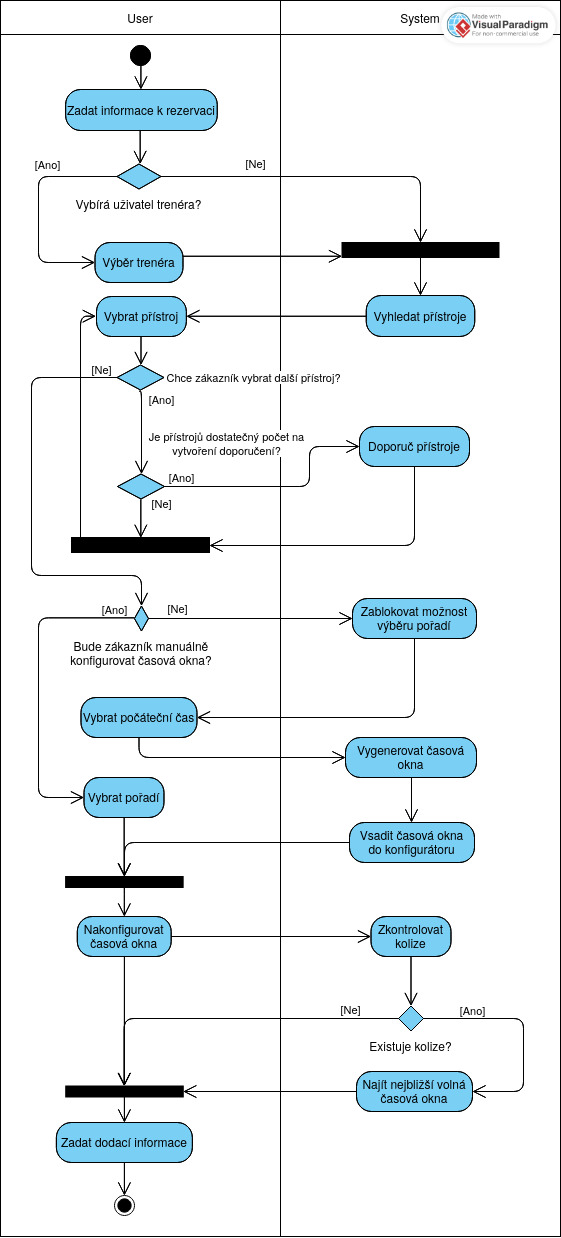
\includegraphics[width=.5\textwidth]{Figures/Bakalarka, rezervace.jpg}
    \caption{Action diagram procesu vytvoření rezervace}
    \label{fig:ReservationActionDiagram}
\end{figure}

\section{Doporučení přístrojů}
Doporučení přístrojů na základě jejich typu je vcelku jednoduché. Nejprve je nutné určit pro jaký typ tréninku se budou přístroje doporučovat. To zajistíme tak, že budeme mít v informaci o možných typech tréninku někde uloženou, konkrétně v databázi. 

Systém tedy projde každý vybraný přístroj, zjistí jaké typy tréninku jsou na přístroji možné a ten, který se vyskytuje ve všech bude považovat za cílový trénink, který zákazník chce navolit. Na základě naleznutého typu tréninku tedy systém najde všechny přístroje, který tento tyt sdílí a podle jejich populaliry vybere několik nejpopulárnějších. 

Problémy s kolizemi v tuto chvíli není potřeba u doporučování přístrojů řešit. Systém nebude mít ve chvíli kdy bude zákazník přístroje vybírat kontext o tom, kdy se trénink bude odehrávat.

\section{Doporučení najbližšího dostupného času}
Doporučení nejbližšího času je již komplexnější. Problematika spočívá v detekci kolizí a v hledání časového okna, které je stejné délky a nekoliduje s žádnou další rezervací a to jak před zvoleným časovým oknem, tak i po něm.

Uživatel bude schopen si také povolit, nebo zakázat kolize na jednotlivých přístrojích. Například je pro systém žádoucí mít neustále povolené kolize na činkách, jelikož jich je mnoho. Kolize se budou řešit úplně stejně jako případy bez kolizí, jen s tím rozdílem, že u kolizí ještě bude systém kontrolovat kapacitu. Pokud bude souběžný počet lidí na jednom přístroji v mezích jeho kapacity, tak systém považuje toto časové okno jako volné; pokud ne, tak ho považuje jako zabrané. Uživatel bude na existující kolizi upozorněn, ale nebude se jednat o stav blokující ho ve vytvoření rezervace.

Systém nejprve načte existující rezervace daného přístroje pro zvolené datum a extrahuje z nich počáteční a koncové časy všech rezervovaných časových oken. Tato okna jsou následně seřazena vzestupně podle počátečního času, čímž vzniká chronologický přehled obsazených intervalů. Před zahájením analýzy systém předpokládá, že uživatelem zadané časové okno splňuje základní validaci – počáteční čas je chronologicky před koncovým časem.

Následně systém porovná vstupní časové okno s uspořádaným seznamem rezervací a identifikuje první interval, který s ním koliduje (překrývá se). Jakmile je kolize detekována, algoritmus vyhledá nejbližší volný interval mezi již existujícími rezervacemi před konfliktním oknem, jehož délka odpovídá nebo přesahuje požadovanou dobu trvání. Stejný postup aplikuje i na intervaly za konfliktním oknem, čímž získá dvě potenciální alternativy: první volné okno před a druhé po původně zvoleném čase.

Pro lepší představu se lze odkázat na diagram \ref{fig:ReservationTimeSuggestionDiagram}. Každá bílá buňka reprezentuje zabraná časová okna, červená ty, se kterými zadaný interval koliduje, šedá ty, která jsou moc krátká, a zelená ty, které jsou vhodné pro doporučení. 

\begin{figure}
    \centering
    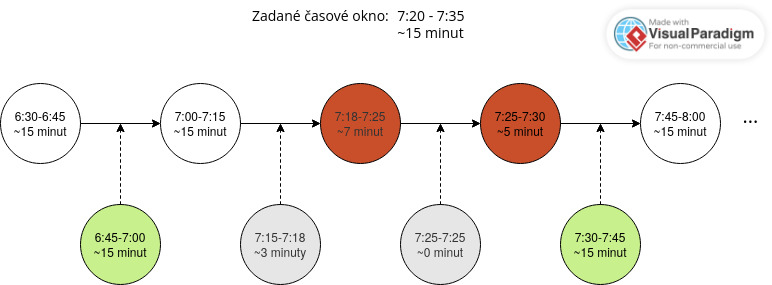
\includegraphics[width=1\textwidth]{Figures/time_suggestion_diagram.jpg}
    \caption{Diagram nalezení nejbližších volných časových oken}
    \label{fig:ReservationTimeSuggestionDiagram}
\end{figure}

\section{Generování času pro trénink}
Generování tréninků je z předem zmíněných možností asi nejkomplexnější. Problematika spočívá v tom, že nejenže musíme najít vhodné časy, ale opět řešit kolize a to vše, aby byl trénink bez prázdných časových oken, ve kterých zákazník nemá zarezervovaný nějaký přístroj. 

Nejprve je potřeba systém v určitých směrech omezit. Například bude velmi složité a neefektivní nechat uživatele zvolit pořadí přístrojů, v tu chvíli by ne jen nabylo řešení na komplexitě, ale také by to omezilo systém v ohledu flexibility, což má být jeden z jeho klíčových aspektů. Zároveň nám zablokování možnosti měnit pořadí otevírá dveře k více flexibilnímu řešení, u kterého může pořadí přístrojů měnit sám systém tak, aby výsledný trénink byl časově efektivní a zabránil tvorbě mezer.

Dále systém umožní uživateli si vypnout, či zapnout kolize s ostatními lidmi, co kolize zapnuté mají. Tyto kolize jsou řešeny podobně jako u Doporučení nejbližšího dostupného času. Nakonec dostaneme od uživatele počáteční čas. 

Generování časových oken bude řešeno pomocí grafů s neváženými směrovými hranami, kde každý vrchol grafu nám reprezentuje časové okno. Výsledkem je několik průchodů tohoto grafu (možností pro uživatele). Graf budeme skládat podle zadaných parametrů, průchod grafem je neměnný. 
\subsection{Tvorba Grafu}

\subsection{Tvorba vrcholů}
Data v grafu vycházejí z využití vybraných přístrojů pro daný den počínaje uživatelem zadaným časem. Je nutné v datech zachovat i ty záznamy, které mají kolize vypnuté, jelikož budou důležité pro tvorbu vrcholů.

Jakmile systém získá záznamy o vytížení přístrojů, je potřeba tato data upravit do požadovaného formátu. Tento formát musí obsahovat počáteční a koncový čas časového okna, který reprezentuje. Dále je potřeba  zachovat informace o přístroji a rezervaci. Dále tato data systém upraví ještě jednou a to tím způsobem, že si doplní záznamy o mezerách, tj. časová okna, přes která nikdo nemá vytvořenou rezervaci pro daný přístroj. Tyto záznamy tedy nebudou obsahovat rezervaci. 

Tyto data budeme tedy následovně upravovat na základě vstupních hodnot poskytnutých uživatelem. Konkrétně, za uživatel povolí kolize s ostatními uživateli, kteří tuto možnost také povolili.

Pokud uživatel kolize nepovolí, tak se nabízí zcela jednoduché řešení. Z předem připravených dat jednoduše odstraníme ty možnosti, které obsahují rezervaci, tj. někdo přes toto časové okno již rezervaci má. Tyto data budou tedy výslednými vrcholy pro tento scénář.

V případě, že uživatel kolize povolí, bude problém o něco složitější. Nejprve z právě těch záznamů, které obsahují rezervaci a zároveň mají kolize povolené, systém musí danou rezervaci odstranit, tímto se z těchto záznamů stanou předem zmíněné mezery. Rezervace, které mají kolize zakázané, musí v datech zůstat. Dále systém projde všechny tyto mezery a spojí je dohromady.
Tímto se nám zmenší počet vrcholů, přes které systém poté bude procházet. Až po spojení mezer systém odstraní záznamy, jež obsahují zbývající rezervace.

Výsledkem obou případů jsou volná časová okna, která jsou pro danou konfiguraci dostupná, právě tyto hodnoty budou hodnotou vrcholů, jež v grafu budou.

\subsection{Tvorba vrcholů}
Pro tvorbu vytvoření hran v grafu se řídí dvěma základními podmínkami.

Následující podmínky využívají 2 vrcholy, vrchol A je právě ten vrchol, ze kterého má směřovat hrana a vrchol B je kandidát na vrchol do kterého hrana směřuje.
\begin{enumerate}
    \item Koncový čas vrcholu B musí být větší, než počáteční čas vrcholu A.
    \item Přístroj asociovaný s vrcholem A nesmí být stejný jako přístroj asociovaný s vrcholem B
\end{enumerate}

Pokud tyto dvě podmínky systém aplikuje na všechna nalezená časová okna, tak výsledkem budou potřebné hrany, skrz které se bude algoritmus pro průchod pohybovat.


\subsection{Průchod grafem}
Na průchod grafem se nabízí spousta možností, jako jsou například: DFS, BFS, Dijkstra a pod. Tyto algoritmy se dají využít na spoustu use-case, ale pro naši implementaci si vystačíme s vlastním řešením.

Průchod grafem bude řešen pomocí rekurze. Princip rozhodování dalšího vrcholu bude jednoduchý. Následující vrchol bude první prvek z množiny vzestupně seřazené podle koncového času, který nebyl dosud navštíven a zároveň neobsahuje přístroj, jenž byl navštíven a časově se do vrcholu vejde.

Průchod grafem je vizualizován v obrázqku \ref{fig:graph_walk}. S ohledem na přehlednost byly v tomto příkladu vynecháno zobrazení všech možných hran mezi všemi vrcholy. Zelenou barvou jsou vyhrazeny hrany, jež jsou vybrány pro další průchod. Vpravo od grafu jsou informace k přístrojům a současný čas.

\begin{figure}
	\centering
	\subfloat[Hrany pro první vrchol přístroje s identifikátorem 1\label{fig:graph_walk_1}]
	{
		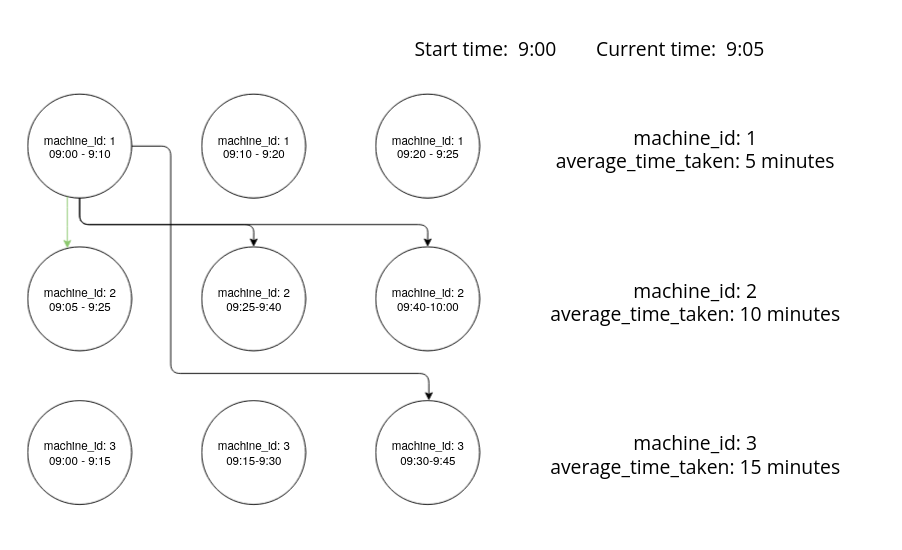
\includegraphics[width=0.9\textwidth]{Figures/graph-node-1.png}
	}
	\vspace{3em} % make more space
	\subfloat[Hrany pro vybraný vrchol v grafu\label{fig:graph_walk_2}]
	{
		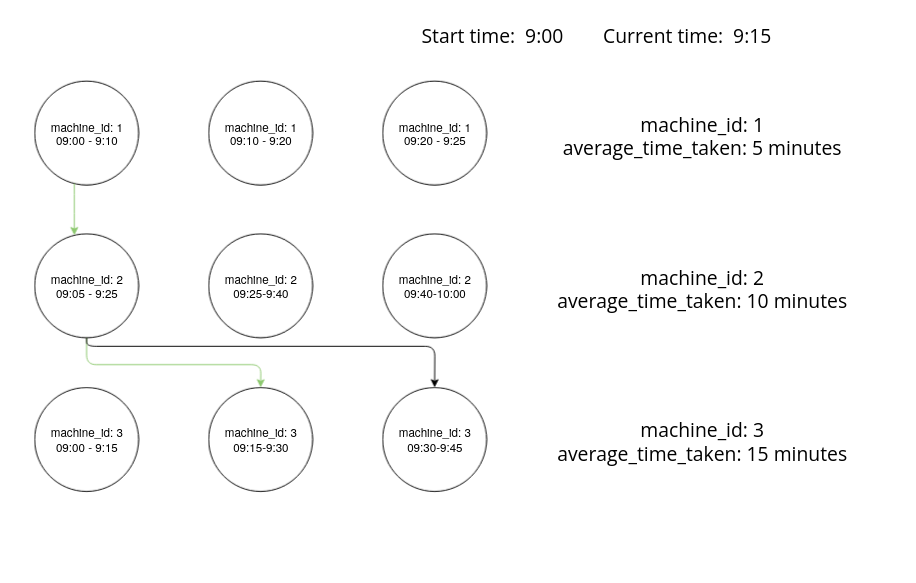
\includegraphics[width=0.9\textwidth]{Figures/graph-node-2.png}
	}
	\caption{Ukázkový průchod grafem pro 3 vybrané přístroje s počátečním časem 9:00}
	\label{fig:graph_walk}
\end{figure}
